\chapter{Modular Run-Time}

\section{Objectives}

When thinking about creating a run-time from the scratch, one has to think mainly about two things:

\begin{itemize}
  \item{\bf{Speed}} The run-time is the core of every app that uses it. The speed of the apps using the run-time is greatly dependent on the speed of the run-time, the method dispatch in particular.
  \item{\bf{Flexibility}} The run-time should be as flexible as possible. It should be easy to port the framework to other platforms, and even to kernel space. You should be able to add custom features to the run-time without modifying the run-time's source code - just adding another source code file and possibly registering it on the fly without the need to even recompile the run-time.
\end{itemize}

The main objective of this work is to create a prototype of a completely new run-time that will have no dependencies on any external libraries, not even the POSIX layer, thus allowing the developer to easily set up his own run-time from different modules.

Also, no constructs that require any OS support (dynamic loader, standard OS libraries, etc.) will be used. This means, that constructs such as \verb=static __thread= (which creates a new copy of the variable declared for each thread created) or \newline{} \verb=__attribute__((constructor))= (which marks the function to be called by the dynamic loader right after the binary has been loaded) can be used either.

In its way, the run-time will be a bare skeleton, which will be ready to be extended for a particular system. As I have decided not to use any compiler-specific extensions, the \verb=constructor= attribute in particular, a question arises, who or what will initialize the run-time.

On systems that do support the constructor functions, this can be easily solved by compiling the run-time with an additional file which will declare and implement a constructor, as can be seen in the \verb=posix.c= file, which is included with the run-time as an extra, which demonstrates how to add support for your operating system.

In a real-world scenario, of course, it cannot be assumed that every program's \verb=main= function will start by feeding the run-time with necessary function pointers and calling the run-time initializer. For example, on \verb=*nix=\footnote{Most Unix-based systems, cannot be guaranteed that this will work on all of the systems.} systems, this can be easily solved by compiling the library with a single \verb=.c= file which has a function populating the setup structure with system-specific functions. As can be seen in the aforementioned \verb=posix.c= file.

This only solves a half of the problem. Who is responsible for calling the \verb=_objc_posix_init= function if your system doesn't support constructor functions? If it is possible to tie the run-time with the OS more tightly, the answer is the dynamic loader. If this isn't the case, then a few options emerge:

\begin{itemize}
  \item{\bf{Use a special \verb=main= function}} Instead of implementing the main function in the program itself, implement it inside the run-time and make it call an external \verb=objc_main= function, which would get to be implemented in the program. It is similar to start of a C program, where the \verb=start= function is called, which initializes some C global variables and then calls the \verb=main= function.
  \item{\bf{Add hooks to class registration}} Second option is to add a check into the class creating/registering functions if the run-time has already been initialized (a global variable may be used for this) and if not, call the initializing function and continue. Class registration function seems like a good place to add such a hook as it doesn't make sense to call any other functions if no classes have been registered with the run-time. Also, such a check does cost something (an \verb=if= statement), so it is not suitable for any function that gets called more often.
\end{itemize}

Now that the initialization has been figured out, even on systems that do not support constructors, another question comes up - what about the on-the-fly customization? What if I want to customize the run-time at the beginning of my program? Here's a few examples a person might want to change:

\begin{itemize}
\item{\bf{Example 1: Lock-less run-time}}
In a single-threaded application (or applications, where you know that Objective-C code will be used only in one thread), there is no need for any locking whatsoever. All of the existing implementations require some locking, even though they are using read-lock-free structures, such as sparse arrays that do not support deleting.

But even so, any \verb=@synchronized(obj)= code is translated to actually lock a mutex associated with \verb=obj=, be it either a mutex from a lock pool in the traditional run-times, or a mutex that is associated just with \verb=obj= in the \'Etoil\'e run-time. This can speed up both loading of the application and code execution.

\item{\bf{Example 2: Kernel usage}}

To get the existing run-times working in a kernel of an operating system might be tricky, depending on how much the kernel is POSIX-compatible. But even so, the \verb=malloc= functions and others usually are just wrappers around kernel allocators, which slows down allocation of all structures within the run-time.

Using the modular run-time, it is be possible to change the allocator with a simple function-pointer assignment.

\item{\bf{Example 3: Benchmarking}}

The modularity that will be introduced by this work will allow anyone to explore changes in the speed of the run-time simply by changing internal data structures used to hold the class list, selector list and caching. This may help the future development of the run-time.

\end{itemize}

Logically, there needs to be some sort of a line after which the run-time cannot be modified as it would lead to inconsistency - for example changing the deallocator after some objects have been already allocated may lead to memory leaks or crashes as the new deallocator will not recognize that particular memory. The following section describes how to set up the run-time.

\section{Run-time Setup}

As has been mentioned before, the run-time has been designed to be as flexible as possible. This means that all possible dependencies had to be removed, as well as all assumptions about the underlying OS, or whether the run-time is running in user space, or kernel space.

The run-time, however, needs a way to allocate memory, locks, and so on, which are system-specific tasks. The intention behind this run-time is to completely separate these dependencies, so that porting the run-time to another platform is as easy as providing a single file containing all the necessary resources.

There are basically two ways of doing so:

\begin{itemize}
\item{\bf{Inline Functions}}
The first one is very similar to what the other run-time implementations have done - create a header file that contains multiple static inline functions that implement all the OS-specific calls required by the run-time.

This approach to the platform-independence problem has one advantage and one disadvantage. The obvious disadvantage is that you can perform compile-time changes only. Once the run-time has been compiled, there is no way to change, for example, the allocator without performing some wild hackery exchanging the \verb=malloc= function pointer using the dynamic loader API.

The advantage, on the other hand, is definitely speed. There is no extra cost associated with calling these system APIs as the functions get inlined.

\item{\bf{Function Pointers}}
Another approach is to create a setup structure that consists of function pointers, which are then called by the run-time. This has the opposite advantages and disadvantages as inlining functions.

The advantage is that the run-time can be compiled without knowing the functions at all and then every program can decide which allocators to use, etc. Or if there is enough support from the dynamic loader, the dynamic loader can decide which functions to use to populate the run-time setup based on some binary flags.

The disadvantage here, on the other hand, is speed. While the function itself has to be called anyway, it is possible that the function types used in the run-time do not match function types in your system. You then need to create a proxy function that converts the parameters.

For example, the read/write lock functions are made to be compatible with the POSIX \verb=pthread_rwlock_*= functions (as can be seen in \verb=extras/posix.c=), which return an \verb=int= containing a possible error value, or zero if the call was successful. In the same manner, the run-time may assume that if the function pointer returns zero, the call was successful. If the OS you are porting the run-time to doesn't return anything, or returns a different value than zero for success, you need to create a proxy function that calls the system function and then returns some value accordingly. This, however, costs an extra function call.

\end{itemize}

Assuming that function pointers are used, you might want to disable all locks in your program as has been described in \textbf{Example 1} above. Even though most operating systems no-op all mutex-related function unless the program is running as multi-threaded. You may, however, be running a multi-threaded application with Objective-C code running in just one thread. Then it may be useful to no-op all the locking functions manually.

If there already is a function that fills all the function pointers, like the one in the \verb=posix.c= example, you need to modify the mutex pointers after the \verb=_objc_posix_init()= is called, as otherwise your change to the function pointers would get overwritten, yet before \verb=objc_runtime_init()= is called, as afterwards, any attempt to modify the run-time setup will result in abort.

Again, several options emerge:

\begin{itemize}
  \item{\bf{With compiler and dynamic loader support}} If enough support is possible from both, just like the \verb=constructor= attribute, other attributes, such as \verb=objc_constructor= and \verb=objc_modifier= could be used, where the constructor would get called first, in our example the \verb=_objc_posix_init= and the modifiers would follow.
  \item{\bf{Without compiler and dynamic loader support}} As the previous option requires a lot of support from both the compiler and dynamic loader, it is unlikely to be used in less common operating systems, which this work is trying to target. For this reason, the run-time supports registering initializer functions that get called within \verb=objc_runtime_init=. Because the run-time has no way to allocate new memory, the number of such initializer functions needs to be limited to 32.
  
  This, again, poses a question when to call \verb=objc_runtime_init=. And the answer is simple. The run-time places a check in the \verb=objc_class_create= function and if the run-time hasn't been initialized, it gets initialized. So what if you call another function before the initialization? The program is likely to crash since it doesn't make much sense to call any other function without having registered at least one class.
  
  Note though that this is only to support systems with absolutely no support of anything described above, where the user himself would otherwise need to call the \verb=objc_runtime_init= function at the beginning of \verb=main= - which he still can, but it is redundant. If, however, for whatever reason, it is required to init the run-time at another time, it is possible to just call the \verb=objc_runtime_init= function manually. It can be called multiple times, however, only calling it the first time does anything. Note that registering an initializer after the runtime has been initialized aborts the program, though.
\end{itemize}

\subsection{Implementation}

The run-time prototype that is part of this work is designed to support both solutions - function pointers and static inline functions. Hence if you decide that you want to choose speed over flexibility and dynamic nature of the run-time, you can do so.

The key to this is the \verb=os.h= header file. An \verb#if-#else= divides the file into two parts, one for the inlining support, second one for the function pointers support.

When compiling the run-time, you can switch between these two simply by redefining the \verb=OBJC_USES_INLINE_FUNCTIONS= value - \verb=0= for function pointers, \verb=1= for inline functions. This can be done in the \verb=Makefile= as can be seen in the sample \verb=Makefile= supplied.

\paragraph{Inlining}

The first part of the \verb=os.h= header file is the part that should be used for static inline functions. A rough sketch of how this should be used has been included:

\begin{verbatim}
#if TARGET_MY_OS
  #include "os-my-os.h"
#else
  #error "This OS isn't supported at the moment."
#endif
\end{verbatim}

You should hence create your own header file for that particular OS and include it in the run-time source files. The obvious disadvantage here is that you need to supply all necessary functions at the compile time.

The following list of functions needs to be defined:

\begin{itemize}
  \item{\bf{objc\_alloc}} Memory allocator.
  \item{\bf{objc\_zero\_alloc}} Memory allocator that fills the allocated memory with zeroes.
  \item{\bf{objc\_dealloc}} Memory deallocator.
  \item{\bf{objc\_abort}} Aborts the executions of the program.
  \item{\bf{\emph{objc\_log}}} Logs supplied format string.
  \item{\bf{objc\_rw\_lock\_create}} Creates a read-write lock.
  \item{\bf{objc\_rw\_lock\_rlock}} Locks the lock as read-only.
  \item{\bf{objc\_rw\_lock\_wlock}} Locks the lock as read/write.
  \item{\bf{objc\_rw\_lock\_unlock}} Unlocks the lock.
  \item{\bf{objc\_rw\_lock\_destroy}} Deallocates the lock.
  \item{\bf{\emph{objc\_class\_holder\_create}}} Creates a structure that registers classes.
  \item{\bf{\emph{objc\_class\_holder\_insert}}} Adds a class pointer to the structure.
  \item{\bf{\emph{objc\_class\_holder\_lookup}}} Looks up a class pointer for name.
  \item{\bf{\emph{objc\_selector\_holder\_create}}} Creates a structure that registers selectors.
  \item{\bf{\emph{objc\_selector\_holder\_insert}}} Inserts a selector.
  \item{\bf{\emph{objc\_selector\_holder\_lookup}}} Looks up a selector.
  \item{\bf{\emph{objc\_array\_create}}} Creates an array.
  \item{\bf{\emph{objc\_array\_append}}} Appends an item to an array.
  \item{\bf{\emph{objc\_array\_get\_enumerator}}} Returns an array enumerator.
  \item{\bf{\emph{objc\_cache\_create}}} Creates a cache for dynamic dispatch.
  \item{\bf{\emph{objc\_cache\_destroy}}} Destroys the cache structure.
  \item{\bf{\emph{objc\_cache\_fetch}}} Fetches a method for selector.
  \item{\bf{\emph{objc\_cache\_insert}}} Inserts a method into the cache.
\end{itemize}

When using static inline functions, all of these need to be implemented. To use the default implementation of functions that are marked italic in the list above, you may use the \verb=array-inline.h= and \verb=holder-inline.h= header files that are included in the \verb=extras= directory.

For a detailed description of each function, see the section about function pointers.

\paragraph{Function Pointers}

If you decide to use function pointers, you don't need to modify the run-time source code at all. The second part of the \verb=os.h= header file is filled with \verb=#define=s that fetch the corresponding function pointer. For example:

\begin{verbatim}
#if OBJC_USES_INLINE_FUNCTIONS

  /* ... */

#else

  #include "private.h"

  #define objc_alloc objc_setup.memory.allocator

  /* ... */

#endif

\end{verbatim}

The run-time defines a private \verb=objc_setup= global variable in \verb=runtime.c= and exports it in \verb=private.h=:
 
\begin{verbatim}
objc_runtime_setup_struct objc_setup;
\end{verbatim}

While the user has no direct access to this structure as it is exported in a private header (and the \verb=os.h= header doesn't get exported as well), the run-time itself can access it directly for the sake of speed to eliminate unnecessary function calls that would serve just as proxy calls. The user doesn't have a direct access to the structure only as a security precaution, so that the structure cannot be modified from the outside during the program execution, but the user is free to get the setup structure using the \verb=objc_runtime_get_setup= function, which copies over the whole setup structure. The user can then cache this structure for performance, so that he doesn't have to fetch it each time he wants to access a run-time function.

You can view the structure below:

\begin{verbatim}
typedef struct {
  objc_setup_memory_t memory;
  objc_setup_execution_t execution;
  objc_setup_sync_t sync;
  
  objc_setup_logging_t logging;
  
  objc_setup_class_holder_t class_holder;
  objc_setup_selector_holder_t selector_holder;
  objc_setup_array_t array;
  objc_setup_cache_t cache;
} objc_runtime_setup_t;
\end{verbatim}

The structure contains a set of structures, each containing a set of related functions. For example, the \verb=objc_setup_memory_t= structure:

\begin{verbatim}
typedef struct {
  objc_allocator_f allocator;
  objc_deallocator_f deallocator;
  objc_zero_allocator_f zero_allocator;
} objc_setup_memory_t;
\end{verbatim}

This allows the modularity of the run-time. One can, at the beginning of his program (as has been described above), modify all of those pointers using setter functions declared in \verb=ftypes.h=. After the runtime has been initialized, however, the whole structure is sealed off changes using those setter functions to prevent any data corruption (as some data structures may be already initialized, changing these functions would most likely lead to bad memory access crashing the program). Using any of the setter functions after the run-time has been initialized will cause the program to be aborted.

A description of each section of the setup structure can be found below:

\paragraph{Memory}

As the run-time needs new memory for dynamic object creation, an allocator is needed. All existing run-times use \verb=malloc=, which, however, ties them to systems that use malloc.

The Modular Run-Time lets you specify your own allocator, which can, for example, be just a wrapper around \verb=malloc= adding some debug logging, or a completely different allocator, e.g.\ a kernel allocator as has been mentioned before. It can also be just the \verb=malloc= function itself, as the function type takes just one argument - the size of the memory required and returns a \verb=void*= pointer.

Sometimes, the memory acquired should be filled with zeros - just as the \verb=calloc= function would do, however, it is called \verb=zero_allocator= in this run-time. Also, unlike the \verb=calloc= function, the \verb=zero_allocator= takes only one argument - the size of memory. It can be easily declared as \verb=calloc(1, size)=.

When the run-time is done with memory it has allocated, it will deallocate it using the deallocate function, which has the same signature as the POSIX \verb=free= function.

\paragraph{Execution}

This part of the structure contains function pointers (in current version of the run-time only one) to functions dealing with the execution of the program itself - it is commonly said that there is no software without bugs - hence it is sometimes necessary to abort the program execution if the program gets into an inconsistent point, or a point where illegal arguments are passed to the environment (for example, setting the run-time setup structure to NULL), hence it contains an \verb=objc_abort= function, which aborts the run of the program. Unlike the regular \verb=abort= function, this one takes an additional argument - the reason why it is being aborted.

\paragraph{Synchronization}

The synchronization structure consists of substructures, or in current state a single one - declaring functions related to read-write locks - it is possible in the future additional synchronization-related functions, such as mutex, condition variables, etc.

\subparagraph{Read-Write Locks} The run-time currently uses only read-write locks to prevent concurrent writes to structures, which are mostly read-lock-free. The structure contains functions that create locks, dealloc them, r/w lock them or unlock them. The locking and unlocking functions are compatible with \newline{}\verb=pthread_rwlock_*= functions.

\paragraph{Logging}

In a very few cases, the run-time logs some information, that is mostly useful to an Objective-C developer, to see what went wrong. For example, when creating a class with the same name as an existing class, a message is logged that the class with this name already exists. The logging function is compatible with \verb=printf= and by default is filled with a no-op function, so you don't necessarily need to include a logging function in your run-time setup, if you don't want to see any log messages from the run-time.

\paragraph{Class Holder}

The run-time needs to keep track of all classes that are registered with it. To do so, it needs to keep a list in some data structure. As the run-time is designed to be flexible, it doesn't matter what data structure at all.

There is a defined data type \verb=objc_class_holder= which, however, is only a retyped \verb=void *=. The functions included in this structure need to be able to create such a structure, store a class pointer in it and look up a class pointer for a name, where, of course, speed matters as this class lookup function is used whenever a class method is called.

The run-time provides a default implementation of this structure, a very simple hash table with a constant number of fields for the simplicity. It should be most likely replaced by some more sophisticated structure if the run-time were to be used in an environment with hundreds of classes.

\paragraph{Selector Holder}

Just like with classes, the run-time needs to keep track of selectors, for a simple reason - if there is only one selector of the same name within the run-time, you can hash the pointer (when looking up method implementations later on in a cache), instead of reading the selector's name over and over again.

\paragraph{Arrays}

A lot of the code of the traditional run-times is riddled with code that takes care of consistency of dynamically growing arrays (or rather arrays of arrays) - there's a lot of duplicate code for functions related to lists of methods, protocols, etc.\ on each class.

This run-time declares a \verb=objc_array= type, which is again just a retyped \verb=void *=, but can be implemented in any possible way. The run-time includes a working implementation of such an array and installs these function pointers at initialization, unless other pointers are provided.

The default implementation is a linked list, which keeps track of its first and last object. It also includes a lock for insertion, however, as no delete operation is allowed, the lock doesn't need to be locked for reading.

To enable fast iteration over the array, an enumerator is returned, which contains a \verb=next= field, pointing to the next node. If your implementation does not use a linked list, it is a good idea to store the items in such a wrapper anyway and link them together, so that the run-time can iterate over your structure in a fast manner without knowing any details about its internal structure and implementation.

\paragraph{Cache}

As has been noted several times before, almost any language with dynamic dispatch uses some sort of a cache so that it doesn't have to climb the whole class hierarchy to find a method implementation of a method that is only implemented on the root class.

The caching mechanism is described in a greater detail in the Caching section below. 

If you want to disable the caching mechanism altogether, just replace the cache creator and fetch functions with functions that return \verb=NULL=, and the insert and destroy functions with a no-op function.

\section{Class}

At the core of the run-time lies a structure representing a class. Like the \'Etoil\'e run-time, this run-time doesn't provide a class pair - a class and its meta-class, but only a single class object that contains class methods as well. While it abandons the Smalltalk similarities, it provides greater flexibility, allowing the Objective-C class structure to be used for other languages as well.

\subsection{Structure of a Class}

The class structure begins in the traditional fashion with a pointer to its superclass - the \verb=isa= pointer. This pointer is followed by the class name, class methods and instance methods. Both class methods and instance methods use the \verb=objc_array= structure, which is a list of lists of \verb=Method=s, just like in the other run-times 

// TODO: cache, ivars

\section{Caching}

\section{Extensibility of Classes}

While the other run-times allow the user to specify extra space when allocating both a class and an object, it is very limiting as if you want to add this extra space, you need to replace the \verb=+alloc= method of \verb=NSObject=, but even so, it will not affect all classes in the run-time as not all objects are subclasses of \verb=NSObject= (e.g.\ \verb=NSProxy=).

This is why the modular run-time has introduced class extensions which allow developers to extend the run-time capabilities dynamically. Class extensions can be compared to the run-time delegates. The class extensions must get registered using the \verb=objc_class_add_extension()= function before the run-time gets initialized.

This function has a single argument: a pointer to a \verb=objc_class_extension= structure:

\begin{verbatim}
  typedef struct _objc_class_extension {
    struct _objc_class_extension *next_extension;

    void(*class_initializer)(Class, void*);
    void(*object_initializer)(id, void*);
    void(*object_deallocator)(id, void*);
  
    unsigned int extra_class_space;
    unsigned int extra_object_space;
  
    unsigned int object_offset;
} objc_class_extension;
\end{verbatim}

The first field, \verb=next_extension= is a pointer to the next extension as the run-time keeps class extensions in a linked list. The run-time populates this field automatically.

This field is followed by three function pointers:

\begin{itemize}
  \item \verb=class_initialize= - this function gets called each time a class is registered with the run-time using \verb=objc_finish_class()=. This is the place where the extra space, to which a pointer is passed as the second argument, should get populated and initialized.
  
  \item \verb=object_initializer= - any time an object is allocated, this function gets called in order to initialize the extra space in the object (again, the second argument is a pointer to the extra space within the structure).
  
  \item \verb=object_deallocator= - before the object gets deallocated, each class   extension is provided an option to deallocated any dynamically allocated structures.
\end{itemize}

These pointers are followed by three unsigned integers. The first two declare how much space is requested by this class extension for the class and object structures.

The last field is populated by the run-time, when it is being initialized and tells the extension what is the offset in the extra space for this particular extension. When multiple extensions are installed, the extra space is divided among all the extensions. The following image illustrates this scenario: \newline{}

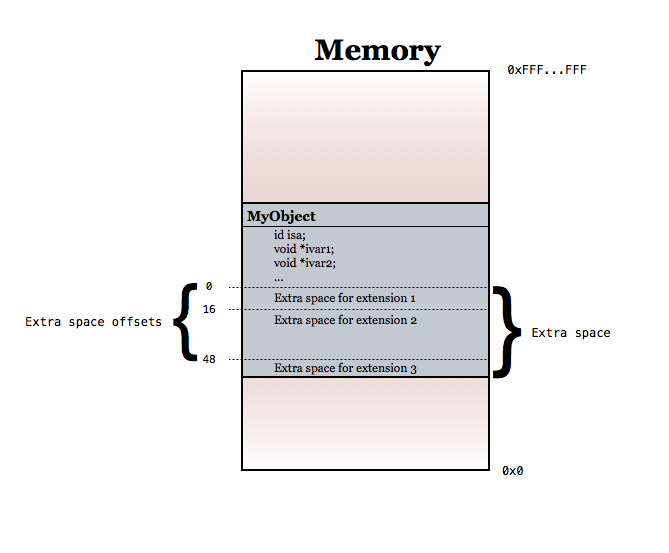
\includegraphics[width=120mm]{img/class_extensions.png}

While it allows to extend the classes with new functionality, for example properties, or ARC (the \verb=object_deallocator= can do all the automatic deallocations), it poses an issue at the compile time - how much extra space should be left? The compiler needs to know the size of the class structure to generate.

One option is to re-allocate all classes with the extra space and copy over all pointers of the class internal structures (it is enough to copy over pointers as the memory will be kept alive). Assuming 1000 classes in a larger application, each class having 64 bytes + those extra bytes, this gives 64 kB of extra memory per application. While this isn't that much nowadays, it would slow down the application launch.

Other option is to dynamically allocate the extra space for each class, so the class structure stays of the same size, with the extra space being outside of the structure itself. This allows to add class functionality without the compiler support and without recompiling any previous classes (note that this applies only to classes - when allocating objects, we can compute the object size as it is not allowed to add class extensions after the run-time has been initialized).

There is an example bundled with the run-time: associated objects (see \verb=extras/associated_objects.c=).

\subsection{Associated Objects}

Since OS X 10.6, Apple's run-time allows to simulate addition of variables to an object using associated objects\footnote{http://developer.apple.com/library/ios/#documentation/cocoa/conceptual/objectivec/ chapters/ocAssociativeReferences.html}. It allows you to specify an object for a key (which is \verb=void*=). Simply said, each object has a hash map, where it stores objects.

With the class and object extensions, it is fairly easy to achieve. The class itself doesn't need to be modified at all, hence the \verb=class_initializer= may be \verb=NULL= or a no-op function and \verb=extra_class_space= should be set to 0.

The \verb=extra_object_space= can be set to \verb=sizeof(void*)= in case you want to allocate the hash-table structure dynamically, or something else, if you want to inline the structure.

If you want to lazily create the hash-table, the \verb=object_initializer= can be \verb=NULL= or a no-op function as well and the \verb=object_deallocator= should simply deallocate the hash-table structure if it were ever created.

Then you can create some getter and setter functions for associated objects. To access the hash-table from an \verb=id object=, you can use code similar to the following:

\begin{verbatim}
  // Static declaration of the extension
  static objc_class_extension 
      associated_objects_extension = { ... }

  // At the beginning, the extension gets added to the run-time
  objc_class_add_extension(&associated_objects_extension);

  // Hash table is retrieved
  void *hashtable = ((void*)id) + id->isa->instance_size 
        + associated_objects_extension.object_extra_space_offset;
        
  // Do something with the hashtable
\end{verbatim}

\subsection{Categories}

\subsection{Performance}
Just like anything, even adding class extension effects the performance somehow. If no extensions are installed in the run-time, the objects are created directly. If extensions get installed, the extension list needs to be iterated and for each extension, one extra function call is performed. This iteration itself doesn't change the asymptotic complexity as the number of class extensions is constant number, usually a very small one. The only thing that can effect the performance is the object initializer function itself.

To speed things up even more for extensions that lazy-initialize their structures (as described in the Associated Objects example), the run-time allows for any of the function pointers to be \verb=NULL= (this includes the \verb=object_deallocator= if your extension doesn't have to allocate dynamically any structures and hence doesn't need to deallocate any as well).

\section{Dynamic Dispatch}

\section{Internal Classes}
\subsection{MRString}

\section{Ports}
\subsection{Windows 3.11}
\subsection{HeSiVa}
